% ViT-Micro on Atalla — team note + data dump (informal layout).
% Build (from atalla-graph/):
%   python3 docs/vit_micro/generate_writeup_figures.py
%   cd docs/vit_micro && pdflatex vit_micro_writeup.tex   % run twice for longtable
\documentclass[10pt,letterpaper]{article}
\usepackage[margin=1in]{geometry}
\usepackage[document]{ragged2e}
\usepackage{graphicx}
\usepackage{booktabs}
\usepackage{longtable}
\usepackage{float}
\usepackage{subcaption}
\usepackage{microtype}
\usepackage{hyperref}
\usepackage{caption}
\usepackage{enumitem}
\usepackage{titlesec}

\hypersetup{colorlinks=true,linkcolor=blue,urlcolor=blue}
\setlength{\parskip}{0.4em}
\setlength{\parindent}{0pt}
\setcounter{secnumdepth}{-1}

% Flat section headings = same body size, left-aligned
\titleformat{\section}{\bfseries\normalsize\RaggedRight}{}{0pt}{}
\titlespacing*{\section}{0pt}{1.1ex plus .2ex}{0.5ex plus .1ex}

% Captions: body-sized, left-aligned (not “report” centered blocks)
\captionsetup{
  font=normalsize,
  labelfont=bf,
  format=plain,
  justification=raggedright,
  singlelinecheck=false,
}
\captionsetup[subfigure]{
  font=normalsize,
  labelfont=bf,
  justification=raggedright,
  singlelinecheck=false,
}

\begin{document}
\RaggedRight

% Title block: same size as body, no centered title page
\noindent\textbf{ViT-Micro on Atalla — measured schedule, DMA, instruction mix}\\
\textit{Team notes, April 2026}
\medskip

\noindent\textbf{Summary.}\ 
We report static and dynamic metrics for ViT-Micro ($B{=}1$, $T{=}32$, $D{=}32$) from \texttt{run\_graph.py} validate plus the functional simulator: schedule sparsity, SDMA bytes, retired-instruction mix by mnemonic class, and per-layer cosines vs.\ BF16 PyTorch.
\textit{Chained} means tensors move through Python's \texttt{activation\_cache} so each emulated op sees the previous emulator output. Attention is \texttt{atalla\_sdpa} with \texttt{ATALLA\_SDPA\_FLASH=1}: the fused flash kernel is compiled and run on the functional sim---there is no NumPy or PyTorch attention substitute in this path. NumPy short-circuits the emulator for \texttt{gelu} (vector-lane limit) and, with the default \texttt{ATALLA\_FFN\_ADD\_NUMPY=1}, for the 2048-wide FFN bias \texttt{add} after the hidden projection; set \texttt{ATALLA\_FFN\_ADD\_NUMPY=0} to force the AtallaC add image for that layer (known mismatch vs.\ ref on the current sim for that shape). Residual and other $1024$-element adds use the C kernel.
We tag claims as Tier~1 (simulator counts), Tier~2 (bytes + SP0/SP1 naming for GEMM CSV columns), or off-paper sketches---Tier~3 tiling art is out of this PDF.
The main empirical punch is the scalar-heavy retired-instruction mix (Table~\ref{tab:retire-mix}) plus brutal static schedule sparsity (Tables~\ref{tab:schedule-aggregate}--\ref{tab:slot-hist}).

\medskip
\noindent\textbf{Pipeline (how to read the tables).}\ 
PyTorch FX is lowered in \texttt{run\_graph.py}; supported ops emit C, compile through AtallaC $\rightarrow$ assembly $\rightarrow$ \texttt{build\_compiler.compile\_asm} (\texttt{schedule\_program} packs VLIW rows), and the functional simulator runs the \texttt{.in} image. Regenerate the artifacts and this PDF with (from \texttt{atalla-graph/}):
\texttt{ATALLA\_SDPA\_FLASH=1 python3 run\_graph.py --model vit\_micro --mode validate --validate-inputs chained}
\texttt{--metrics-json out/graph/vit\_micro\_metrics.json --layer-metrics-csv out/graph/vit\_micro\_layer\_metrics.csv}
then \texttt{python3 docs/vit\_micro/generate\_writeup\_figures.py} and \texttt{pdflatex} as in the header comment.
Metrics land in \texttt{out/graph/vit\_micro\_metrics.json} and \texttt{out/graph/vit\_micro\_layer\_metrics.csv} after validate.

\begin{itemize}[nosep,leftmargin=1.2em]
  \item \textbf{Tier~1:} packet/slot stats from the static image; dynamic packets + retired ops from the sim; SDMA bytes; FLOP model; per-layer cosines on emulated nodes.
  \item \textbf{Tier~2:} CSV \texttt{reuse\_R\_A\_gemm}/\texttt{reuse\_R\_W\_gemm} only mean $A$/$W$ if the emitted kernel matches that bank story---check each \texttt{.c}.
  \item Table~\ref{tab:schedule-aggregate} last row and per-node $\mathrm{AI}_{\mathrm{ld}}$ are model ratios (FLOPs / SDMA bytes), not hardware roofline AI.
\end{itemize}

\section{Findings}

\medskip
\noindent\textbf{Retired instructions} (Table~\ref{tab:retire-mix}).\ 
Scalar ALU + scalar GMEM dominate dynamic retirements; GEMM/systolic is a few percent---so today’s compiled kernels burn most committed ISA slots on scalar bookkeeping and scalar memory, not the MAC array. Buckets come from \texttt{misc/instruction\_retire.py} (mnemonic classes), not a PMU.

% -*- tex -*- auto-generated by docs/vit_micro/generate_writeup_figures.py
% Regenerate:  (from atalla-graph/) python3 docs/vit_micro/generate_writeup_figures.py

\begin{table}[H]
\raggedright
\small
\caption{\textbf{Measured.} Dynamic retired instruction mix (all emulated kernels). One count per non-\texttt{nop.s} op; buckets follow \texttt{misc/instruction\_retire.py} (mnemonic-based; not hardware-classified). Scalar ALU plus scalar GMEM dominate this run; GEMM/systolic is a small fraction.}
\begin{tabular}{@{}l r r@{}}
\toprule
Class & Count & \% of retired ops \\
\midrule
GEMM / systolic & 2,720 & 2.27\% \\
Vector ALU (.vv/.vi/.vs) & 10,209 & 8.53\% \\
Vector mem (vreg.ld/st) & 15,380 & 12.85\% \\
SDMA (scpad) & 585 & 0.49\% \\
Move / convert & 1,568 & 1.31\% \\
Scalar ALU (other) & 53,209 & 44.45\% \\
Scalar GMEM (lw/sw) & 28,660 & 23.94\% \\
Branch / control & 7,369 & 6.16\% \\
\midrule
\textbf{Total (retired ops)} & \textbf{119,700} & 100.00\% \\
\bottomrule
\end{tabular}
\label{tab:retire-mix}
\end{table}


\medskip
\noindent\textbf{Static schedule} (Tables~\ref{tab:schedule-aggregate}, \ref{tab:slot-hist}).\ 
Most static packet rows are empty of real ops before NOP fill; on rows with $\geq 1$ real op, mean slot fill is still $\sim$27\% (Table~\ref{tab:schedule-aggregate})---order one live op per four-slot row.
At most one vector + one memory op per packet, and control takes whole rows, so “heavy” co-issue in a mixed row has a rough 50\% structural ceiling; observed $\sim$27\% is already below that, so not all slack is “the ISA’s fault.” We don’t split forced vs.\ schedulable gap here.
Table~\ref{tab:slot-hist} is the histogram of real-op counts per static row.

% -*- tex -*- auto-generated by docs/vit_micro/generate_writeup_figures.py
% Regenerate:  (from atalla-graph/) python3 docs/vit_micro/generate_writeup_figures.py

\begin{table}[H]
\raggedright
\small
\caption{Static instruction image (aggregated over emulated kernels). A packet row is four slots. \textbf{Empty rows} have no real op before \texttt{nop.s} fill. Last row: ISA-weighted FLOPs / SDMA BF16 bytes---\textit{not} hardware roofline AI.}
\begin{tabular}{@{}l r@{}}
\toprule
Metric & Value \\
\midrule
Total static packet rows & 4,250 \\
Rows with $\geq 1$ real instruction & 4,250 (100.0\%) \\
\textbf{Empty rows} & \textbf{0} (\textbf{0.0\%}) \\
\midrule
Slot fill (all rows) & 27.92\% \\
Slot fill (non-empty rows only) & 27.92\% \\
Dynamic slot fill (retired / dyn.\ packets) & 28.05\% \\
\midrule
Total FLOPs (model) & 1,082,053 \\
DMA bytes loaded & 246,400 \\
\quad SP0 / SP1 loads & 191,104 / 55,296 \\
DMA bytes written & 43,008 \\
\quad SP0 / SP1 stores & 24,576 / 18,432 \\
FLOPs / DMA (ld$+$st), model & 3.739 \\
\bottomrule
\end{tabular}
\label{tab:schedule-aggregate}
\end{table}


\begin{table}[H]
\raggedright
\small
\caption{Histogram: how many real instructions occupy each static packet row (summed across kernels).}
\begin{tabular}{@{}c r r@{}}
\toprule
\# real ops in row & Count & Share \\
\midrule
$1$ & 3,832 & 90.16\% \\
$2$ & 347 & 8.16\% \\
$3$ & 64 & 1.51\% \\
$4$ & 7 & 0.16\% \\
\bottomrule
\end{tabular}
\label{tab:slot-hist}
\end{table}


\medskip
\noindent\textbf{Templates, DMA, retire mix} (Figures~\ref{fig:concentration}, \ref{fig:instr-mix}).\ 
Fig.~\ref{fig:template}: cumulative dynamic packet share by template (fused SDPA $\sim$54\% of dynamic packets in a typical flash run; LayerNorm and $32{\times}32{\times}32$ GEMMs split most of the remainder).
Fig.~\ref{fig:dma}: SDMA bytes per node (attention and FFN GEMMs dominate at this scale).
Fig.~\ref{fig:instr-mix}: same buckets as Table~\ref{tab:retire-mix} per template; LN leans vector-ALU vs.\ GEMM shapes, in line with higher $\eta_{\mathrm{st}}$ on LN rows in Table~\ref{tab:per-layer}.

\begin{figure}[H]
  \noindent
  \begin{subfigure}[t]{0.49\linewidth}
    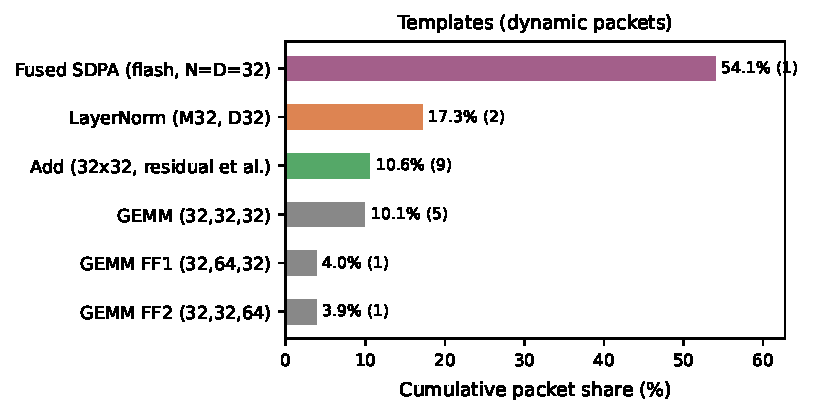
\includegraphics[width=\linewidth]{fig_template_rollup.pdf}
    \caption{Dynamic packet share by template.}
    \label{fig:template}
  \end{subfigure}\hfill
  \begin{subfigure}[t]{0.49\linewidth}
    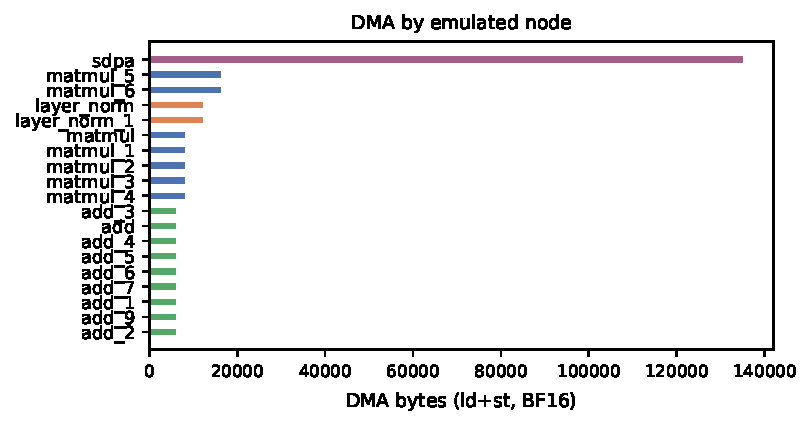
\includegraphics[width=\linewidth]{fig_dma_bytes_by_layer.pdf}
    \caption{DMA bytes (loads + stores) per node.}
    \label{fig:dma}
  \end{subfigure}
  \caption{Measured concentration (Tier~1).}
  \label{fig:concentration}
\end{figure}

\begin{figure}[H]
  \noindent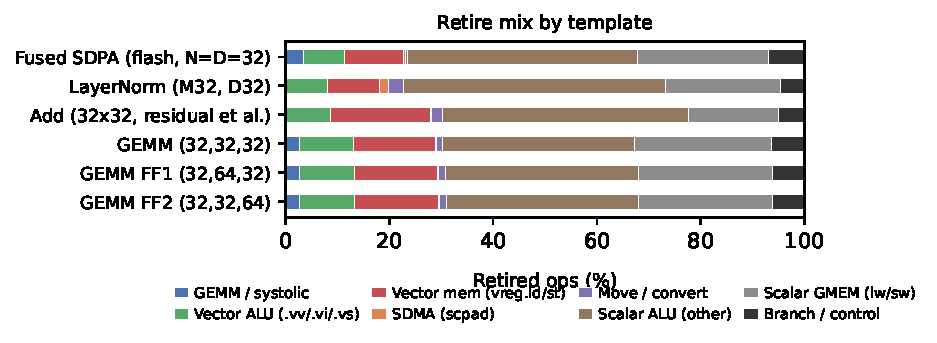
\includegraphics[width=0.88\linewidth]{fig_template_instruction_mix.pdf}
  \caption{Measured. Retired-op mix by template.}
  \label{fig:instr-mix}
\end{figure}

\medskip
\noindent\textbf{Per-node} (Table~\ref{tab:per-layer}).\ 
Per-op cosines vs.\ BF16 ref are high for most emulated nodes; the chained end-to-end cosine is dominated by attention and the wide FFN stages (GELU $+$ optional NumPy bias add) and is $\sim$0.98 in a typical \texttt{ATALLA\_SDPA\_FLASH=1} run with the default NumPy GELU and FFN add paths (see validate console \texttt{cos=})---not a tight ``paper'' match without tightening those paths.
$\eta_{\mathrm{st}}$ is $\sim$28\% on this run; LayerNorm blocks differ from pure GEMM templates in vector vs.\ scalar retire mix (Table~\ref{fig:instr-mix}), not from higher MAC throughput.

% -*- tex -*- auto-generated by docs/vit_micro/generate_writeup_figures.py
% Regenerate:  (from atalla-graph/) python3 docs/vit_micro/generate_writeup_figures.py

\begin{flushleft}
{\footnotesize
\begin{longtable}{@{}l l c r r r r r r r@{}}
\caption[Per-node metrics]{Per-node metrics (emulator layers): Pkt\% = share of dynamic packets; $\eta_{\mathrm{st}}$ = static slot fill (non-\texttt{nop.s} / all static slots); AI$_{\mathrm{ld}}$ = model FLOPs / SDMA bytes loaded---not hardware AI.\protect\footnotemark}\label{tab:per-layer}\\
\toprule
Name & Op & Map & Pkt\% & $P_{\mathrm{stat}}$ & $\eta_{\mathrm{st}}$ & Bytes & FLOPs & AI$_{\mathrm{ld}}$ & $\cos$ \\
\midrule
\endfirsthead
\caption[]{Per-node metrics (continued)}\\
\toprule
Name & Op & Map & Pkt\% & $P_{\mathrm{stat}}$ & $\eta_{\mathrm{st}}$ & Bytes & FLOPs & AI$_{\mathrm{ld}}$ & $\cos$ \\
\midrule
\endhead
\midrule
\multicolumn{10}{r}{\small\itshape Continued on next page}\\
\endfoot
\bottomrule
\endlastfoot
matmul & matmul & $32\times32\times32$ & 2.01 & 319 & 27.3\% & 8256 & 74326 & 11.97 & 1.00000 \\
add\_3 & add & $32\times32$ & 1.18 & 116 & 28.2\% & 6144 & 4470 & 1.09 & 1.00000 \\
add & add & $32\times32$ & 1.18 & 116 & 28.2\% & 6144 & 4470 & 1.09 & 1.00000 \\
layer\_norm & layernorm & LN $32\times32$ & 8.65 & 319 & 29.2\% & 12288 & 31336 & 3.06 & 0.99999 \\
matmul\_1 & matmul & $32\times32\times32$ & 2.01 & 319 & 27.3\% & 8256 & 74326 & 11.97 & 0.99999 \\
add\_4 & add & $32\times32$ & 1.18 & 116 & 28.2\% & 6144 & 4470 & 1.09 & 0.99999 \\
matmul\_2 & matmul & $32\times32\times32$ & 2.01 & 319 & 27.3\% & 8256 & 74326 & 11.97 & 0.99999 \\
add\_5 & add & $32\times32$ & 1.18 & 116 & 28.2\% & 6144 & 4470 & 1.09 & 0.99999 \\
matmul\_3 & matmul & $32\times32\times32$ & 2.01 & 319 & 27.3\% & 8256 & 74326 & 11.97 & 0.99999 \\
add\_6 & add & $32\times32$ & 1.18 & 116 & 28.2\% & 6144 & 4470 & 1.09 & 0.99999 \\
sdpa & atalla\_sdpa & --- & 54.11 & 335 & 28.9\% & 135232 & 310248 & 2.33 & 0.25027 \\
matmul\_4 & matmul & $32\times32\times32$ & 2.01 & 319 & 27.3\% & 8256 & 74326 & 11.97 & 0.44980 \\
add\_7 & add & $32\times32$ & 1.18 & 116 & 28.2\% & 6144 & 4470 & 1.09 & 0.67970 \\
add\_1 & add & $32\times32$ & 1.18 & 116 & 28.2\% & 6144 & 4470 & 1.09 & 0.98122 \\
layer\_norm\_1 & layernorm & LN $32\times32$ & 8.65 & 319 & 29.2\% & 12288 & 31336 & 3.06 & 0.98049 \\
matmul\_5 & matmul & $32\times64\times32$ & 3.95 & 319 & 27.3\% & 16512 & 148638 & 11.97 & 0.97919 \\
matmul\_6 & matmul & $32\times32\times64$ & 3.94 & 319 & 27.3\% & 16512 & 148635 & 11.97 & 0.98182 \\
add\_9 & add & $32\times32$ & 1.18 & 116 & 28.2\% & 6144 & 4470 & 1.09 & 0.98380 \\
add\_2 & add & $32\times32$ & 1.18 & 116 & 28.2\% & 6144 & 4470 & 1.09 & 0.98164 \\
\end{longtable}
}
\end{flushleft}

\footnotetext{Tier~2: CSV \texttt{reuse\_R\_A\_gemm}/\texttt{reuse\_R\_W\_gemm} map SP0/SP1 loads to $A$/$W$ by emitter convention only; audit each \texttt{.c} before reuse claims.}

\section{Scope and next steps}

\begin{itemize}[nosep,leftmargin=1.2em]
  \item \textbf{Scale:} $T{=}D{=}32$ is still toy vs.\ real ViT shapes---don’t extrapolate without re-running.
  \item \textbf{Compiler:} scalar retirements + scalar GMEM (Table~\ref{tab:retire-mix}); slot slack vs.\ structure (Table~\ref{tab:schedule-aggregate}).
  \item \textbf{Validation:} bring GELU and/or the 2048-wide FFN add fully on-chip for stricter chained E2E; flash SDPA already runs on the sim. Audit SP0/SP1 per GEMM before trusting \texttt{reuse\_R\_*\_gemm}.
  \item \textbf{Instrumentation:} split non-empty-row waste; optional Tier~2 pass over emitted \texttt{.c}.
  \item Tier~3 tiling slides live elsewhere unless tied to new counters.
\end{itemize}

\end{document}
